% Setup -------------------------------

\documentclass[a4paper]{article}
\setcounter{secnumdepth}{3}
\setcounter{tocdepth}{3}

\usepackage{hyperref}
\usepackage{indentfirst}

\usepackage{graphicx}
\usepackage[export]{adjustbox}
\usepackage{float}

% Encoding
%--------------------------------------
\usepackage[T1]{fontenc}
\usepackage[utf8]{inputenc}
%--------------------------------------

% Portuguese-specific commands
%--------------------------------------
\usepackage[portuguese]{babel}
%--------------------------------------

% Hyphenation rules
%--------------------------------------
\usepackage{hyphenat}
%--------------------------------------

% References (BibTeX)
%--------------------------------------
\usepackage[backend=bibtex,style=numeric,sorting=ynt]{biblatex}
\usepackage[autostyle=true]{csquotes}
\addbibresource{Report.bib}
%--------------------------------------

% Capa do relatório

\title{
	Sistemas Distribuídos em Larga Escala
	\\ \Large{\textbf{Trabalho Prático}}
	\\ -
	\\ Mestrado em Engenharia Informática
	\\ Universidade do Minho
}
\author{
	\begin{tabular}{ll}
		\textbf{Grupo nº 1}
		\\
		\hline
		PG41080 & João Ribeiro Imperadeiro
        \\
		PG41081 & José Alberto Martins Boticas
		\\
        PG41091 & Nelson José Dias Teixeira
	\end{tabular}
}

\date{\today}

\begin{document}

\maketitle

% Introdução

\section{Introdução} \label{sec:Introduction}
\large{
	O presente relatório descreve o desenvolvimento do projeto de cariz prático da unidade curricular de Sistemas Distribuídos em Larga Escala.
	Neste trabalho é requerida a implementação de um dos algoritmos de agregação distribuída disponíveis no documento de suporte ao enunciado do mesmo \parencite{article}.
	Após a implementação do algoritmo escolhido, é posteriormente solicitado o teste do mesmo no simulador desenvolvido ao longo do semestre do presente ano letivo.

	Tal como é mencionado nas referências bibliográficas \parencite{ref} e \parencite{article}, a agregação de dados distribuídos desempenha um papel bastante importante na concepção de diversos sistemas escaláveis uma vez que possibilita a determinação descentralizada de propriedades globais significativas, 
	que posteriormente podem ser utilizadas para direcionar a execução de outras aplicações distribuídas.
	Vários algoritmos de agregação distribuída foram propostos ao longo dos últimos anos, exibindo propriedades diferentes em termos de precisão, 
	desempenho e de métricas de comunicação. No entanto, muitas dessas abordagens não possuem caraterísticas relacionadas com a tolerância de faltas. 
	Desta forma, no âmbito de sistemas distribuídos, este grupo de trabalho viu-se interessado em implementar um dos algoritmos com esta propriedade.

	Relativamente à estrutura deste relatório, é exibido o algoritmo escolhido, apresentando o conceito e a implementação intrínsecos ao mesmo. 
	Para além disso, são evidenciados alguns aspetos relativos ao simulador utilizado para proceder à realização de testes do algoritmo em causa, efetuando finalmente uma análise dos resultados obtidos.
}

\section{Algoritmo} \label{sec:Algorithm}
\large{
	Dos algoritmos de agregação distribuída presentes no documento referenciado no enunciado deste trabalho prático \parencite{article}, optou-se pela escolha do algoritmo \textbf{\textit{flow updating}}.
	Este, ao nível de comunicação, é classificado como não estruturado, inserindo-se na categoria \textit{gossip} que, por sua vez, diz respeito à forma como as mensagens são disseminadas pela rede de comunicação.
	Quanto à perspetiva computacional, este algoritmo tem como objetivo a computação iterativa de médias parciais que, ao longo do tempo, convergem para um determinado valor.
	Esta última técnica permite também a derivação de outras funções de agregação (como por exemplo, \textit{count} ou \textit{sum}), de acordo com as combinações dos valores inicialmente instanciados.

	Uma das razões que levou este grupo a escolher este algoritmo foi a capacidade do mesmo em tolerar a injeção de faltas transientes. 
	Esta última caraterística é bastante importante sobretudo no que diz respeito à perda de mensagens trocadas na rede de comunicação.
	Com pequenas alterações, é ainda possível que o algoritmo suporte falhas de membros, falhas permanentes de ligações e mudanças de vizinhança.
	Para além destas vantagens associadas ao contexto de sistemas distribuídos, este algoritmo possui não só um melhor desempenho quando comparado com os outros da mesma classe, como também possibilita uma computação mais precisa de valores.
	Por fim, a execução do algoritmo em causa é independente da topologia do roteamento de rede.

	No \hyperref[sec:Analysis of results]{4º capítulo} deste documento são devidamente clarificados todos os resultados obtidos após a implementação do algoritmo escolhido, discutindo-se a veracidade das propriedades mencionadas acima.

	\subsection{Conceito} \label{subsec:Concept}
	O algoritmo \textit{flow updating} difere de outros propostos para o mesmo problema no sentido em que não se procede ao envio de mensagens complexas que, posteriormente, são armazenadas e disseminadas.
	Em contraste, faz uso do conceito de fluxo (no sentido da teoria de grafos), atualizando-o com recurso ao valor inicial e à contribuição de fluxos de outros nós vizinhos, sendo que o fluxo é simétrico nos extremos de cada ligação. Por isto, a soma das médias de cada um dos nós deve manter-se constante.
	Assim, partilha-se apenas o fluxo com os vizinhos, sendo que a perda de uma destas mensagens não implica uma falha grave.
	A intuição é que a simetria pode ser quebrada, se for possível garantir que uma mensagem chegará no futuro e a restabeleça.

	Importa realçar que existem duas versões do algoritmo. A primeira assenta no envio de mensagens com recurso a \textit{broadcast} (\textit{N} para \textit{N}) enquanto que a segunda enquadra-se no envio de mensagens em \textit{unicast} (1 para 1).


	\subsection{Implementação} \label{subsec:Implementation}
	Tal como foi referido no fim do \hyperref[subsec:Concept]{subcapítulo anterior}, foram implementadas duas versões distintas do algoritmo em questão.
	À semelhença do que foi elaborado durantes as aulas práticas desta unidade curricular, estas duas versões foram implementadas na linguagem \texttt{Python}.
	Para cada uma das mesmas são exibidos os respetivos detalhes computacionais e, ainda, um pequeno esquema relativo ao seu pseudocódigo.

		\subsubsection{\textit{Broadcast}}
		Relativamente a esta abordagem, criou-se uma classe para representar um nó do grafo, com o nome \texttt{flowUpdatingBroad}, que contém as seguintes informações no seu estado:
		\begin{itemize}
			\item um dicionário \textit{f} que contém os fluxos desses nós para os seus vizinhos;
			\item um dicionário \textit{e} que contém as estimativas que recebeu dos seus vizinhos;
			\item o seu valor inicial \textit{v};
			\item a lista dos seus vizinhos;
			\item as mensagens acumuladas de uma ronda;
			\item um inteiro \textit{timeout} que representa a duração pré-estabelecida de cada ronda.
		\end{itemize}

		Esta classe contém ainda as seguintes funções:
		\begin{itemize}
			\item \texttt{gen\_message} - devolve a lista de mensagens a serem enviadas nessa ronda, incluindo uma mensagem especial de \textit{timeout}, dirigida ao próprio nó e que representa o fim de uma ronda;
			\item \texttt{state\_transition} - executada em reação à mensagem de \textit{timeout}, ou seja, no fim da ronda, por forma a calcular as novas estimativas e fluxos dos vizinhos, bem como os próprios;
			\item \texttt{calculate\_estimate} - executada pelo método anterior e que corresponde ao valor calculado durante a transição de estado, ou seja, devolve a nova estimativa para o valor objetivo.
		\end{itemize}

		Dito isto, divulga-se de seguida uma figura representativa do pseudocódigo associado a esta versão:
		\begin{figure}[H]
			\centering
			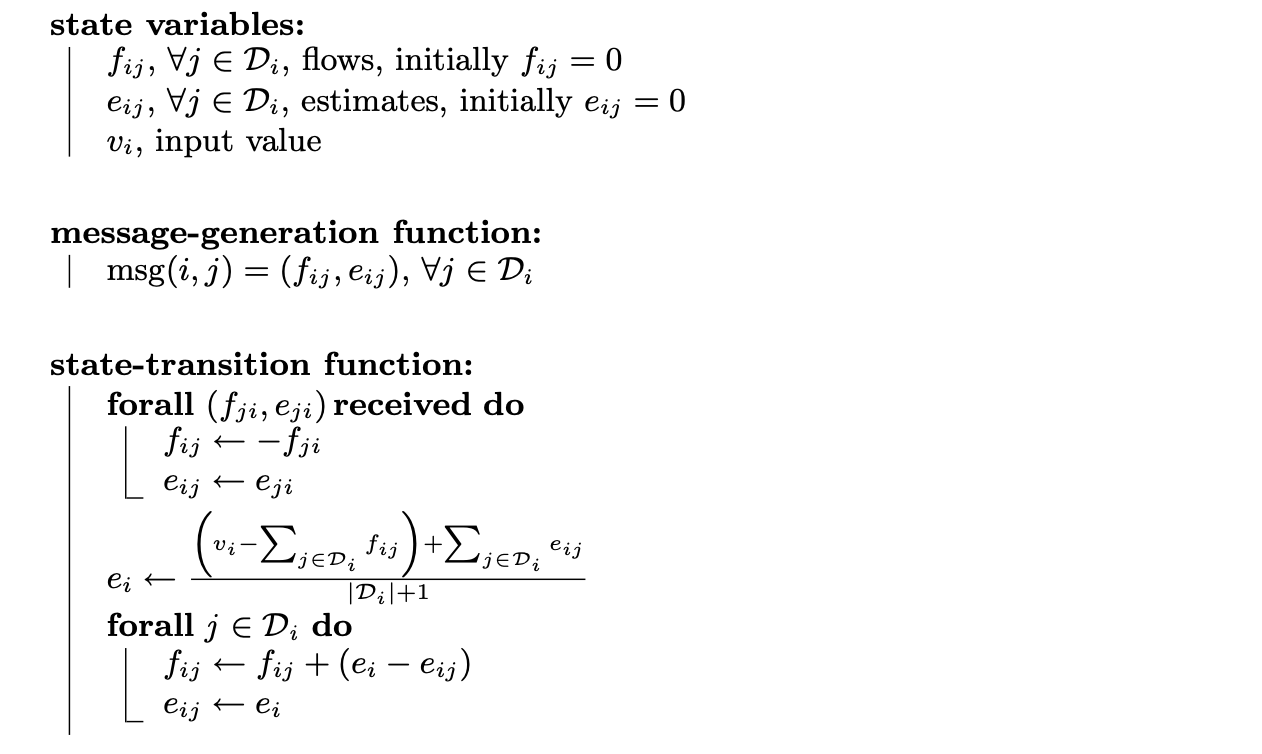
\includegraphics[width=1.0\textwidth, frame]{Images/Broadcast - Pseudocode.png}
			\caption{Pseudocódigo do algoritmo \textit{Flow Updating} (\textit{broadcast})}
			\label{fig:1}
		\end{figure}

		\subsubsection{\textit{Unicast}}
		Quanto a esta versão, concebeu-se, da mesma forma, uma classe para representar um nó do grafo, com o nome \texttt{flowUpdatingUni}, que contém as mesmas informações, no seu estado, que as indicadas acima, para a classe de \textit{Broadcast}.
		Para além destas, têm ainda um inteiro representativo do identificador do vizinho escolhido, sendo que o mesmo é selecionado pela função \texttt{chooseNeighbor}, que, tal como o nome transparece, devolve aleatoriamente o identificador de um dos vizinhos.

		As funções desta classe são as mesmas que as expostas anteriormente na classe \textit{broadcast}, com as seguintes alterações:
		\begin{itemize}
			\item \texttt{gen\_message} - calcula apenas uma mensagem para o vizinho \textit{k}, em vez de todos os vizinhos, e a mensagem especial de fim de ronda;
			\item \texttt{state\_transition} - calcula apenas a estimativa e o fluxo do vizinho \textit{k};
		\end{itemize}

		Expõe-se agora um diagrama alusivo ao pseudocódigo desta versão:
		\begin{figure}[H]
			\centering
			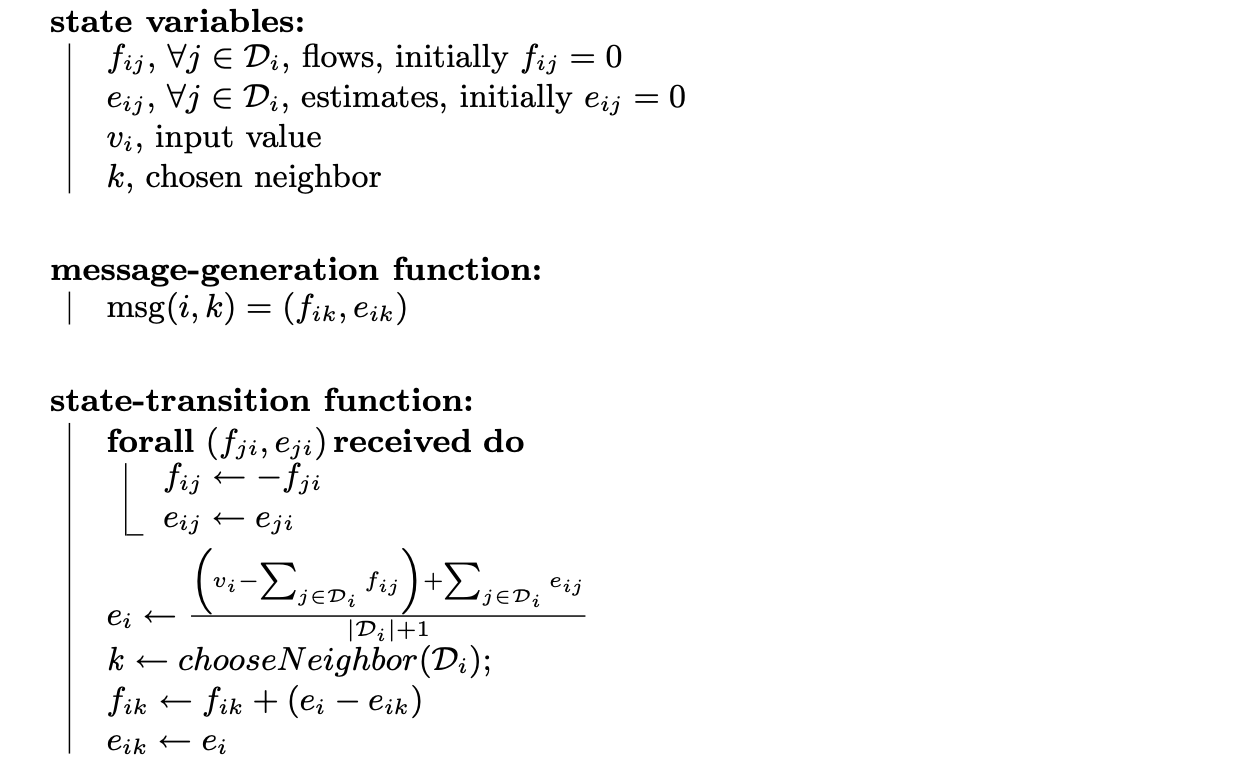
\includegraphics[width=1.0\textwidth, frame]{Images/Unicast - Pseudocode.png}
			\caption{Pseudocódigo do algoritmo \textit{Flow Updating} (\textit{unicast})}
			\label{fig:2}
		\end{figure}
}

\section{Simulador} \label{sec:Simulator}
\large{
	...
}

\section{Análise de resultados obtidos} \label{sec:Analysis of results}
\large{
	Os resultados da avaliação obtidos, quando comparados com outras abordagens de \textit{averaging}, revelaram que os superam em termos de complexidade temporal (maior desempenho) e ao nível do número de mensagens trocadas (\textit{overhead}).
}

\section{Conclusão} \label{sec:Conclusion}
\large{
	Este algoritmo tolera a perda substancial de mensagens (\textit{link failures}), enquanto outros algoritmos concorrentes da mesma categoria podem ser afetados por uma única mensagem perdida.
}

\printbibliography[heading=bibintoc]

\end{document}